%!TEX root = Report.tex

% Overvej at kalde dette afsnit "Experimentation" eller "Testing"
% 
% vis hvornår det virker og hvornår det ikke virker. 
% Se at det virker når vi regnede med at det virkede.
% 
% Hvad tester vi?
% Hvordan tester vi det?
% Virkede det efter hensigten?
% Hvorfor/hvorfor ikke?
% Er der nok testing?
% Hvordan kan man lave mere testing?
% Er der andre måder vi kunne have testet på? (fordele og ulemper ved det)

\subsection{Testing the tracking software with real ants}

Having solved the problem of finding an ant on a single image and integrated our software with the XY-plotter and camera, this section focus on testing how the integrated solution works with a video feed of an ant running arond in a controlled environment.\\

The test were performed in a ordinary office environment, with the plotter placed on a table. The room were only litten by daylight, and we used the setup explained in section (REF HANDLING ANTS), with a petridish filled with ground material surround by water, as can be seen in Figure (INSERT FIGURE WITH IMAGE OF SETUP). According to our experimentation in (INSERT REF TO EXPERIMENTATION) we painted our ant with a white color to have the best possible color for tracking.\\

In the following we will show several results of running the software, both where the tracking works as intented, but also situations where the software does not work. We will end this section with a summary of the challenges presented by this real-time testing and suggest possible solutions to the problems and an overall evaluation of how the software together with the plotter an camera performs performs. We will also comment on the important observations done during testing.\\

We will begin by showing several images from the test where the software tracking works. Examples can be seen in Figure \ref{fig:ant_tracking}. We are showin both the final thresholded image, as well as the original image. For this test, the images were contrasted with an $\alpha = 2.0$ and $T = 240$.\\

\begin{figure}
        \centering
        \begin{subfigure}[b]{0.35\textwidth}
                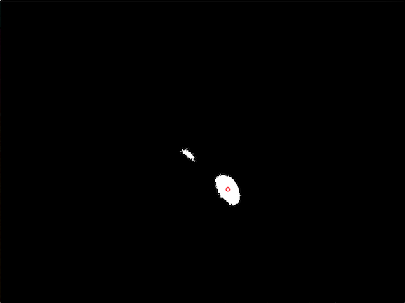
\includegraphics[scale = 0.3]{img/good1t}
                \caption{}
        \end{subfigure}
		\quad
        \begin{subfigure}[b]{0.35\textwidth}
                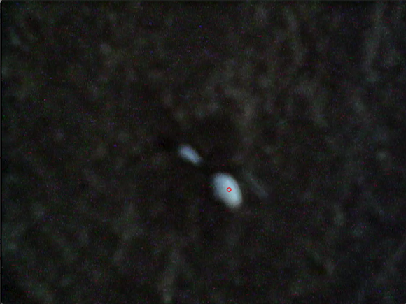
\includegraphics[scale = 0.3]{img/good1}
                \caption{}
        \end{subfigure} \hfill \\ \mbox{}\\
        \begin{subfigure}[b]{0.35\textwidth}
                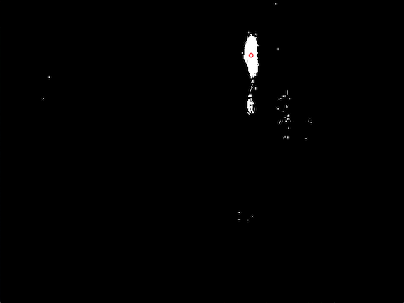
\includegraphics[scale = 0.3]{img/good2t}
                \caption{}
        \end{subfigure}
		\quad
        \begin{subfigure}[b]{0.35\textwidth}
                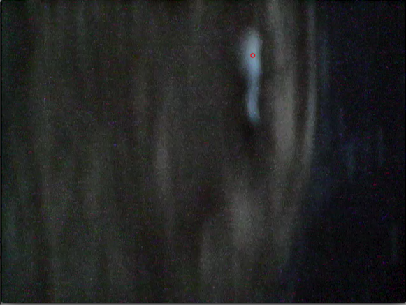
\includegraphics[scale = 0.3]{img/good2}
                \caption{}
        \end{subfigure}\hfill \\ \mbox{}\\
        \begin{subfigure}[b]{0.35\textwidth}
                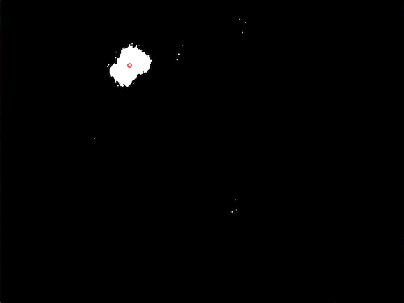
\includegraphics[scale = 0.3]{img/good3t}
                \caption{}
        \end{subfigure}
		\quad
        \begin{subfigure}[b]{0.35\textwidth}
                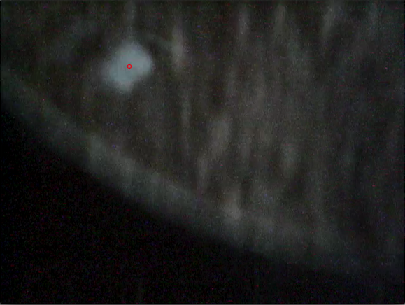
\includegraphics[scale = 0.3]{img/good3}
                \caption{}
        \end{subfigure}\\ \mbox{}\\
        \begin{subfigure}[b]{0.35\textwidth}
                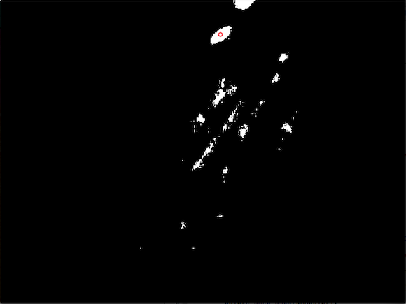
\includegraphics[scale = 0.3]{img/good4t}
                \caption{}
        \end{subfigure}
		\quad
        \begin{subfigure}[b]{0.35\textwidth}
                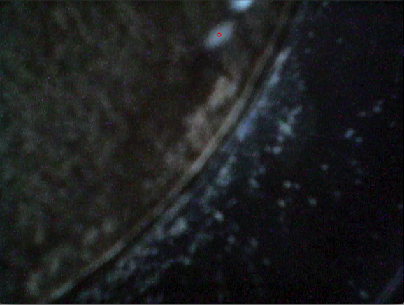
\includegraphics[scale = 0.3]{img/good4}
                \caption{}
        \end{subfigure}
		\caption{Examples of real-time ant tracking.}
		\label{fig:ant_tracking}
\end{figure}

\newpage